\begin{figure}[t]
\centering
\usepgfplotslibrary{groupplots}
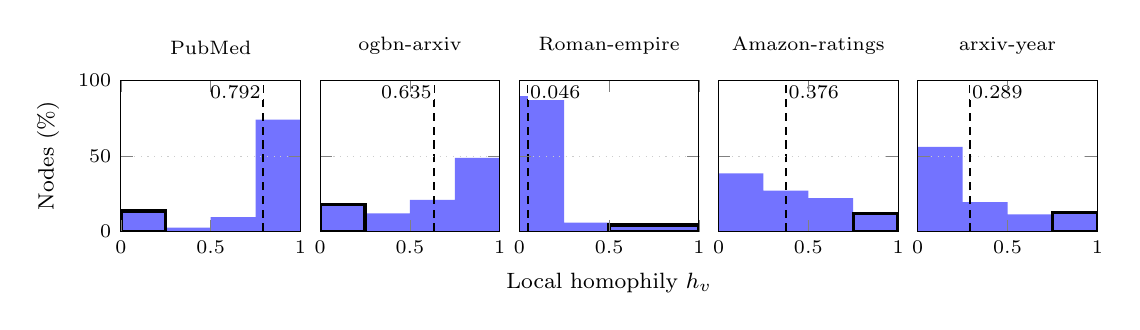
\begin{tikzpicture}
\begin{groupplot}[
    group style={
        group size=5 by 1,
        horizontal sep=0.25cm,
        ylabels at=edge left,
        yticklabels at=edge left
    },
    scale only axis,
    width=2.28cm,
    height=1.92cm,
    xmin=0, xmax=1,
    ymin=0, ymax=100,
    xtick={0,0.5,1},
    ytick={0,50,100},
    tick label style={font=\scriptsize},
    title style={font=\scriptsize},
    label style={font=\footnotesize},
    ymajorgrids=true,
    grid style={dotted,gray!40},
    axis on top,
]

\nextgroupplot[
    title={PubMed},
    ylabel={Nodes (\%)}
]
\addplot+[ybar interval, fill=blue!55, draw=none, mark=none]
coordinates {
    (0,13.7)
    (0.25,2.7)
    (0.5,9.6)
    (0.75,74.1)
    (1,0)
};
\addplot+[ybar interval, fill=blue!55, draw=black, line width=1.2pt, mark=none]
coordinates {(0,13.7) (0.25,0)};
\draw[densely dashed,black,line width=0.7pt]
    (axis cs:0.792,0) -- (axis cs:0.792,100);
\node[font=\scriptsize,anchor=north east,fill=white,inner sep=0.7pt]
    at (axis cs:0.792,98) {0.792};

\nextgroupplot[title={ogbn-arxiv}]
\addplot+[ybar interval, fill=blue!55, draw=none, mark=none]
coordinates {
    (0,17.9)
    (0.25,12.1)
    (0.5,21.1)
    (0.75,48.9)
    (1,0)
};
\addplot+[ybar interval, fill=blue!55, draw=black, line width=1.2pt, mark=none]
coordinates {(0,17.9) (0.25,0)};
\draw[densely dashed,black,line width=0.7pt]
    (axis cs:0.635,0) -- (axis cs:0.635,100);
\node[font=\scriptsize,anchor=north east,fill=white,inner sep=0.7pt]
    at (axis cs:0.635,98) {0.635};

\nextgroupplot[
    title={Roman-empire},
    xlabel={Local homophily \(h_v\)}
]
\addplot+[ybar interval, fill=blue!55, draw=none, mark=none]
coordinates {
    (0,89.6)
    (0.25,6.0)
    (0.5,4.5)
    (1,0)
};
\addplot+[ybar interval, fill=blue!55, draw=black, line width=1.2pt, mark=none]
coordinates {(0.5,4.5) (1,0)};
\draw[densely dashed,black,line width=0.7pt]
    (axis cs:0.046,0) -- (axis cs:0.046,100);
\node[font=\scriptsize,anchor=north west,fill=white,inner sep=0.7pt]
    at (axis cs:0.046,98) {0.046};

\nextgroupplot[title={Amazon-ratings}]
\addplot+[ybar interval, fill=blue!55, draw=none, mark=none]
coordinates {
    (0,38.6)
    (0.25,27.1)
    (0.5,22.2)
    (0.75,12.0)
    (1,0)
};
\addplot+[ybar interval, fill=blue!55, draw=black, line width=1.2pt, mark=none]
coordinates {(0.75,12.0) (1,0)};
\draw[densely dashed,black,line width=0.7pt]
    (axis cs:0.376,0) -- (axis cs:0.376,100);
\node[font=\scriptsize,anchor=north west,fill=white,inner sep=0.7pt]
    at (axis cs:0.376,98) {0.376};

\nextgroupplot[title={arxiv-year}]
\addplot+[ybar interval, fill=blue!55, draw=none, mark=none]
coordinates {
    (0,56.1)
    (0.25,19.6)
    (0.5,11.4)
    (0.75,12.9)
    (1,0)
};
\addplot+[ybar interval, fill=blue!55, draw=black, line width=1.2pt, mark=none]
coordinates {(0.75,12.9) (1,0)};
\draw[densely dashed,black,line width=0.7pt]
    (axis cs:0.289,0) -- (axis cs:0.289,100);
\node[font=\scriptsize,anchor=north west,fill=white,inner sep=0.7pt]
    at (axis cs:0.289,98) {0.289};

\end{groupplot}
\end{tikzpicture}
\caption{Distribution of nodes across local-homophily bins. Bar
widths show the bin intervals and heights show within-dataset percentages.
Dashed lines give mean \(h_v\); thick outlines mark the selected tails.}
\label{fig:local-homophily-bins-tikz}
\end{figure}
